\documentclass[paper=A4, fontsize=11pt, titlepage]{article}

\usepackage[utf8]{inputenc}
\usepackage[T1]{fontenc} 
\usepackage{fourier} 
\usepackage[english]{babel}
\usepackage{graphicx}
\usepackage{amsmath,amsfonts,amsthm} 
\usepackage{fancyhdr} 
\usepackage{titlesec}
\usepackage{multirow}
\usepackage[super]{nth}
\usepackage[pdftex,pdfpagelabels,bookmarks,hyperindex,hyperfigures,hidelinks,linktoc=all]{hyperref}
\usepackage[all]{hypcap}
\usepackage{tikz-timing}[2009/05/15]

\pagestyle{fancy}
\renewcommand{\sectionmark}[1]{ \markboth{#1}{} }
\setlength{\headheight}{24pt}
\fancyhf[HL]{\raisebox{-0.4\height}{
\includegraphics[height=24pt]{fig/udemheader}}}
\fancyhead[HC]{\leftmark}
\fancyhf[HR]{\raisebox{-0.4\height}{
\includegraphics[height=24pt]{fig/esisarheader}}}
\fancyhf[FC]{\thepage}

\titleformat{\section}
{\normalfont\Large\bfseries}{\thesection}{1em}{}
[\normalfont\small\itshape\raggedleft\sectionpostamble\global\let\sectionpostamble\relax]

\numberwithin{equation}{section}
\numberwithin{figure}{section}
\numberwithin{table}{section}

\setlength\parindent{0pt}

\newcommand{\horrule}[1]{\rule{\linewidth}{#1}} 
\newcommand*{\sectionpostamble}{}
\newcommand*{\fromto}[1]{\def\sectionpostamble{#1}}

%%%%%%%%%%%%%%%%%%%%%%%%%%%%%%%%%%%%%%%%%%%%%%%
\begin{document}
\pagenumbering{roman}
  \begin{titlepage}
    \begin{center}
	
\includegraphics[height=0.35\textwidth]{fig/udemlogo}\\
	\vspace{2mm}
	\huge UNIVERSIDAD DE MONTERREY\\
	\vspace{1mm}
	\Large División de Ingeniería y Tecnologías\\
	\vspace{1mm}
	\large Departamento de Inegniería\\
	\vspace{10mm}
	\horrule{1pt} \\[0.4cm]
	\Huge ACTIVITIES REPORT\\ 
	\large Final Evaluation Project\\
	\horrule{2pt} \\[0.5cm]
	\vspace{10mm}
	\Large\raggedright Dr. Jorge de Jesús Lozoya Santos\\
	\normalsize\raggedright Project Assessor\\
	\vspace{10mm}
	\Large\raggedleft Pedro Aguiar\\
	\normalsize\raggedleft Mechatronics Engineering Student\\
	\vspace{20mm}
	\Large\centering\today\\
    \end{center}
  \end{titlepage}

\tableofcontents
\clearpage
\listoffigures
\listoftables
\clearpage
\pagenumbering{arabic}
%%%%%%%%%%%%%%%%%%%%%%%%%%%%%%%%%%%%%%%%%%%%%%%

\fromto{April 23 - May 2}
\section{MEMORANDUM 01}

\subsection{Administrative Process}

There were some pending administrative procedures that are reported here as a reference and information for future UDEM students that could participate in a similar program. Upon my arrival to the laboratory I was taken to Jennyfer DUBERVILLE to check for pending steps at the administrative procedures. The documents that were sent via Internet were checked for possible corrections. These documents are:
\begin{itemize}
	\item Student card.
	\item Copy of the last diploma (mine was from high school).
	\item Copy of my passport.
	\item The contract/agreement (signed by me and the Dean of UDEM's DIT)
\end{itemize}
After reviewing the documents a form was given to my assessor and the rules/regulations (mostly about the use of laboratory's resources such as internet, computers, etcetera) were given to me. I signed of agreement to the rules and declaring the date of arrival to the laboratory. I was reminded I have to pay the "social security" and "civil liability" fees when prompted. I was also informed that for receiving the gratification I have to open a bank account in a French bank and I was told I was going to be contacted with a person that could help me with that.

Finally I was given my authentication credentials which I will be using to connect to the wireless network and to sign in to my computer. My assigned computer was installed and some other restrictions were informed (you can not connect to the wired network, you can not install software other than from Debian's repositories, how to access the schools backed up servers, etcetera).

\subsection{Activities}

%%%%%%%%%%%%%%%%%%%%%%%%%%%%%%%%%%%%%%%%%%%%%%%%%%%%%%%%%%%%%%%%%%%%%%

\subsubsection{Pin selection}
\begin{table}[ht!]
\begin{center}
\begin{tabular}{| c | c | c | c | c | c | c |}
\hline
\multicolumn{1}{|c|}{DCMI}	 & 	\multicolumn{1}{c|}{Pin}	 & 	\multicolumn{1}{c|}{Board} & 	\multicolumn{1}{c|}{Pin}	 & 	\multicolumn{1}{c|}{Board} & 	\multicolumn{1}{c|}{Pin}	 & 	\multicolumn{1}{c|}{Board}\\ \hline
D0	&	PA9	&	Free	&	PC6	&	\scriptsize LCD-TFT \& LCD-RGB	&		&	\\
D1	&	PA10	&	Free	&	PC7	&	\scriptsize LCD-TFT \& LCD-RGB	&		&	\\
D2	&	PC8	&	Free	&	PG10	&	\scriptsize LCD-TFT \& LCD-RGB	&	PE0	&	SDRAM\\
D3	&	PG11	&	\scriptsize LCD-TFT \& LCD-RGB	&	PC9	&	\scriptsize ACP/RF \& Touch panel	&	PE1	&	SDRAM\\
D4	&	PE4	&	Free	&	PC11	&	Free	&		&	\\
D5	&	PD3	&	\scriptsize LCD-TFT \& LCD-RGB	&	PB6	&	SDRAM	&		&	\\
D6	&	PE5	&	Free	&		&		&		&	\\
D7	&	PE6	&	Free	&	PB9	&	\scriptsize LCD-TFT \& LCD-RGB	&		&	\\
HSYNC	&	PA4	&	\scriptsize LCD-TFT \& LCD-RGB	&		&		&		&	\\
VSYNC	&	PB7	&	Free	&	PG9	&	Free	&		&	\\
PXCLK	&	PA6	&	\scriptsize LCD-TFT \& LCD-RGB	&		&		&		&	\\ \hline
\end{tabular}
\caption{Pin options for each DCMI signal according to the microcontroller's datasheet and the peripheral they are connected to at the discovery board.}
\label{tab_boardpin_dcmi}
\end{center}
\end{table}

\begin{table}
\begin{center}
\begin{tabular}{| c | c | c | c | c |}
\hline
\multicolumn{1}{|c|}{Conflicted pin}	 & 	\multicolumn{1}{c|}{LCD TFT}	 & 	\multicolumn{1}{c|}{LCD RGB} & 	\multicolumn{1}{c|}{I/O}	 & 	\multicolumn{1}{c|}{Action}\\ \hline
PA4	&	VSYNC	&	VSYNC	&	I	&	Nothing\\
PA6	&	DB6	&	G2	&	I/O	&	Force input or float\\
PD3	&	DB11	&	G7	&	I/O	&	Force input or float\\
PG11	&	DB11	&	B3	&	I/O	&	Force input or float\\ \hline
\end{tabular}
\caption{Discovery board DCMI non-free pins and the action to trigger at the target device to avoid problems.}
\label{tab_boardpin_dcmi_conflict}
\end{center}
\end{table}

\begin{table}[ht!]
\begin{center}
\begin{tabular}{| c | c | c | c | c |}
\hline
\multirow{2}{*}{Signal}	&	\multicolumn{2}{|c|}{SPI1}		&	\multicolumn{2}{|c|}{SPI4}\\ \cline{2-5}
	&	Posible Pin	&	Datasheet	&	Posible Pin	&	Datasheet	\\ \hline
\multirow{2}{*}{SCK}	&	PA5	&	Free	&	PE12	&	SDRAM	\\
	&	PB3	&	System	&	PE2	&	Free	\\ \hline
\multirow{2}{*}{MOSI}	&	PB5	&	SDRAM	&	PE6	&	Free	\\
	&	PA7	&	ACP/RF	&	PE14	&	SDRAM	\\ \hline
\multirow{2}{*}{MISO}	&	PB4	&	Free	&	PE5	&	Free	\\
	&	PA6	&	LCD-TFT \& LCD-RGB	&	PE13	&	SDRAM	\\ \hline
\multirow{2}{*}{NSS}	&	PA15	&	Touch panel	&	PE11	&	SDRAM \\
	&	PA4	&	LCD-TFT \& LCD-RGB	&	PE4	&	Free \\ \hline
\end{tabular}
\caption{Options for each SPI signal (SPI1 and SPI2) according to microcontroller's datasheet and the peripheral they are connected to on the discovery board.}
\label{tab_boardpin_spi_a}
\end{center}
\end{table}

\begin{table}[ht!]
\begin{center}
\begin{tabular}{| c | c | c | c | c | c | c | c | c |}
\hline
\multirow{2}{*}{Signal}	&	\multicolumn{2}{|c|}{SPI5}		&	\multicolumn{2}{|c|}{SPI6}	\\ \cline{2-5}
	&	Posible Pin	&	Datasheet	&	Posible Pin	&	Datasheet \\ \hline
SCK	&	PF7	&	\scriptsize LCD-TFT \& LCD-SPI \& L3GD20	&	PG13	&	LED \\ \hline
\multirow{2}{*}{MOSI}	&	PF9	&	\scriptsize LCD-TFT \& LCD-SPI \& L3GD20	&	PG14	&	LED \\
	&	PF11	&	SDRAM	&		&	\\ \hline
MISO	&	PF8	&	L3GD20	&	PG12	&	\scriptsize LCD-TFT \& LCD-RGB \\ \hline
NSS	&	PF6	&	Free	&	PG8	&	SDRAM \\ \hline
\end{tabular}
\caption[Options for each SPI signal (SPI5 and SPI6).]{Options for each SPI signal (SPI5 and SPI6) according to microcontroller's datasheet and the peripheral they are connected to on the discovery board.}
\label{tab_boardpin_spi_b}
\end{center}
\end{table}

\begin{table}
\begin{center}
\begin{tabular}{| c | c | c | c | c |}
\hline
Conflicted pin	&	LCD TFT	&	LCD RGB	&	L3GD20 \\ \hline
PF7	&	DCX	&	SCL	&	SCK \\
PF8	&	-	&	-	&	MISO \\
PF9	&	SDA	&	SDI/SDO	&	MOSI \\ \hline
\end{tabular}
\caption{Discovery board SPI5 non-free pins and the signal they carry. It is only necessary to keep the SS pins high for these devices.}
\label{tab_boardpin_spi5_conflict}
\end{center}
\end{table}

\begin{table}[ht!]
\begin{center}
\begin{tabular}{| c | c | c |}
\hline
Pin	&	Peripheral	&	Signal\\ \hline
PA04	&	\multirow{11}{*}{DCMI}	&	HSYNC\\
PA06	&		&	PXCLK\\
PA09	&		&	D0\\
PA10	&		&	D1\\
PB07	&		&	VSYNC\\
PC08	&		&	D2\\
PD03	&		&	D5\\
PE04	&		&	D4\\
PE05	&		&	D6\\
PE06	&		&	D7\\
PG11	&		&	D3\\ \hline
PC01	&	\multirow{3}{*}{GPIO}	&	CS Gyro\\
PC02	&		&	CS LCD\\
PF10	&		&	EN LCD\\ \hline
PC09	&	MCO	&	MCO2\\ \hline
PF06	&	\multirow{4}{*}{SPI5}	&	NSS\\
PF07	&		&	SCK\\
PF08	&		&	MISO\\
PF09	&		&	MOSI\\ \hline
PA05	&	TIM2	&	TIM2\_CH1\\ \hline
\end{tabular}
\caption{Final selections of pins to be used by the application.}
\label{tab_boardpin_final}
\end{center}
\end{table}

%%%%%%%%%%%%%%%%%%%%%%%%%%%%%%%%%%%%%%%%%%%%%%%%%%%%%%%%%%%%%%%%%%%%%%



\subsection{Results}

\subsubsection{Interface PCB between the camera and the raspberry pi.}
\begin{itemize}
	\item Bill of materials shown in table \ref{tab_bompic}.
	\item Due to the high cost of this solution an alternative was proposed.
\end{itemize}

\subsubsection{Microchip alternative.}
\begin{itemize}
	\item A STM32 microcontroller will be used.
	\item The board to be used is the 32F429IDISCOVERY evaluation board.
\end{itemize}

\subsubsection{Study and C implementation of the Hough transform.}
\begin{itemize}
	\item The theory behind the Hough transform was understood.
	\item A traditional Hough transform was implemented using only C language (with very few dependencies).
\end{itemize}

\subsubsection{Bibliographical review of Hough transform applications.}
\begin{itemize}
	\item A bibliographical review was started.
	\item Modifications (and their justification) done to the traditional Hough transform to apply it to real applications were observed.
\end{itemize}


\subsection{Pending}

\begin{itemize}
	\item Camera mount mechanism.
	\item New disparity map shader.
	\item Integration into the multithreaded program.
\end{itemize}

\clearpage

%%%%%%%%%%%%%%%%%%%%%%%%%%%%%%%%%%%%%%%%%%%%%%%

\fromto{May 5 - May 9}
\section{MEMORANDUM 02}

\subsection{Activities}

%%%%%%%%%%%%%%%%%%%%%%%%%%%%%%%%%%%%%%%%%%%%%%%%%%%%%%%%%%%%%%%%%%%%%%

\subsubsection{Pin selection}
\begin{table}[ht!]
\begin{center}
\begin{tabular}{| c | c | c | c | c | c | c |}
\hline
\multicolumn{1}{|c|}{DCMI}	 & 	\multicolumn{1}{c|}{Pin}	 & 	\multicolumn{1}{c|}{Board} & 	\multicolumn{1}{c|}{Pin}	 & 	\multicolumn{1}{c|}{Board} & 	\multicolumn{1}{c|}{Pin}	 & 	\multicolumn{1}{c|}{Board}\\ \hline
D0	&	PA9	&	Free	&	PC6	&	\scriptsize LCD-TFT \& LCD-RGB	&		&	\\
D1	&	PA10	&	Free	&	PC7	&	\scriptsize LCD-TFT \& LCD-RGB	&		&	\\
D2	&	PC8	&	Free	&	PG10	&	\scriptsize LCD-TFT \& LCD-RGB	&	PE0	&	SDRAM\\
D3	&	PG11	&	\scriptsize LCD-TFT \& LCD-RGB	&	PC9	&	\scriptsize ACP/RF \& Touch panel	&	PE1	&	SDRAM\\
D4	&	PE4	&	Free	&	PC11	&	Free	&		&	\\
D5	&	PD3	&	\scriptsize LCD-TFT \& LCD-RGB	&	PB6	&	SDRAM	&		&	\\
D6	&	PE5	&	Free	&		&		&		&	\\
D7	&	PE6	&	Free	&	PB9	&	\scriptsize LCD-TFT \& LCD-RGB	&		&	\\
HSYNC	&	PA4	&	\scriptsize LCD-TFT \& LCD-RGB	&		&		&		&	\\
VSYNC	&	PB7	&	Free	&	PG9	&	Free	&		&	\\
PXCLK	&	PA6	&	\scriptsize LCD-TFT \& LCD-RGB	&		&		&		&	\\ \hline
\end{tabular}
\caption{Pin options for each DCMI signal according to the microcontroller's datasheet and the peripheral they are connected to at the discovery board.}
\label{tab_boardpin_dcmi}
\end{center}
\end{table}

\begin{table}
\begin{center}
\begin{tabular}{| c | c | c | c | c |}
\hline
\multicolumn{1}{|c|}{Conflicted pin}	 & 	\multicolumn{1}{c|}{LCD TFT}	 & 	\multicolumn{1}{c|}{LCD RGB} & 	\multicolumn{1}{c|}{I/O}	 & 	\multicolumn{1}{c|}{Action}\\ \hline
PA4	&	VSYNC	&	VSYNC	&	I	&	Nothing\\
PA6	&	DB6	&	G2	&	I/O	&	Force input or float\\
PD3	&	DB11	&	G7	&	I/O	&	Force input or float\\
PG11	&	DB11	&	B3	&	I/O	&	Force input or float\\ \hline
\end{tabular}
\caption{Discovery board DCMI non-free pins and the action to trigger at the target device to avoid problems.}
\label{tab_boardpin_dcmi_conflict}
\end{center}
\end{table}

\begin{table}[ht!]
\begin{center}
\begin{tabular}{| c | c | c | c | c |}
\hline
\multirow{2}{*}{Signal}	&	\multicolumn{2}{|c|}{SPI1}		&	\multicolumn{2}{|c|}{SPI4}\\ \cline{2-5}
	&	Posible Pin	&	Datasheet	&	Posible Pin	&	Datasheet	\\ \hline
\multirow{2}{*}{SCK}	&	PA5	&	Free	&	PE12	&	SDRAM	\\
	&	PB3	&	System	&	PE2	&	Free	\\ \hline
\multirow{2}{*}{MOSI}	&	PB5	&	SDRAM	&	PE6	&	Free	\\
	&	PA7	&	ACP/RF	&	PE14	&	SDRAM	\\ \hline
\multirow{2}{*}{MISO}	&	PB4	&	Free	&	PE5	&	Free	\\
	&	PA6	&	LCD-TFT \& LCD-RGB	&	PE13	&	SDRAM	\\ \hline
\multirow{2}{*}{NSS}	&	PA15	&	Touch panel	&	PE11	&	SDRAM \\
	&	PA4	&	LCD-TFT \& LCD-RGB	&	PE4	&	Free \\ \hline
\end{tabular}
\caption{Options for each SPI signal (SPI1 and SPI2) according to microcontroller's datasheet and the peripheral they are connected to on the discovery board.}
\label{tab_boardpin_spi_a}
\end{center}
\end{table}

\begin{table}[ht!]
\begin{center}
\begin{tabular}{| c | c | c | c | c | c | c | c | c |}
\hline
\multirow{2}{*}{Signal}	&	\multicolumn{2}{|c|}{SPI5}		&	\multicolumn{2}{|c|}{SPI6}	\\ \cline{2-5}
	&	Posible Pin	&	Datasheet	&	Posible Pin	&	Datasheet \\ \hline
SCK	&	PF7	&	\scriptsize LCD-TFT \& LCD-SPI \& L3GD20	&	PG13	&	LED \\ \hline
\multirow{2}{*}{MOSI}	&	PF9	&	\scriptsize LCD-TFT \& LCD-SPI \& L3GD20	&	PG14	&	LED \\
	&	PF11	&	SDRAM	&		&	\\ \hline
MISO	&	PF8	&	L3GD20	&	PG12	&	\scriptsize LCD-TFT \& LCD-RGB \\ \hline
NSS	&	PF6	&	Free	&	PG8	&	SDRAM \\ \hline
\end{tabular}
\caption[Options for each SPI signal (SPI5 and SPI6).]{Options for each SPI signal (SPI5 and SPI6) according to microcontroller's datasheet and the peripheral they are connected to on the discovery board.}
\label{tab_boardpin_spi_b}
\end{center}
\end{table}

\begin{table}
\begin{center}
\begin{tabular}{| c | c | c | c | c |}
\hline
Conflicted pin	&	LCD TFT	&	LCD RGB	&	L3GD20 \\ \hline
PF7	&	DCX	&	SCL	&	SCK \\
PF8	&	-	&	-	&	MISO \\
PF9	&	SDA	&	SDI/SDO	&	MOSI \\ \hline
\end{tabular}
\caption{Discovery board SPI5 non-free pins and the signal they carry. It is only necessary to keep the SS pins high for these devices.}
\label{tab_boardpin_spi5_conflict}
\end{center}
\end{table}

\begin{table}[ht!]
\begin{center}
\begin{tabular}{| c | c | c |}
\hline
Pin	&	Peripheral	&	Signal\\ \hline
PA04	&	\multirow{11}{*}{DCMI}	&	HSYNC\\
PA06	&		&	PXCLK\\
PA09	&		&	D0\\
PA10	&		&	D1\\
PB07	&		&	VSYNC\\
PC08	&		&	D2\\
PD03	&		&	D5\\
PE04	&		&	D4\\
PE05	&		&	D6\\
PE06	&		&	D7\\
PG11	&		&	D3\\ \hline
PC01	&	\multirow{3}{*}{GPIO}	&	CS Gyro\\
PC02	&		&	CS LCD\\
PF10	&		&	EN LCD\\ \hline
PC09	&	MCO	&	MCO2\\ \hline
PF06	&	\multirow{4}{*}{SPI5}	&	NSS\\
PF07	&		&	SCK\\
PF08	&		&	MISO\\
PF09	&		&	MOSI\\ \hline
PA05	&	TIM2	&	TIM2\_CH1\\ \hline
\end{tabular}
\caption{Final selections of pins to be used by the application.}
\label{tab_boardpin_final}
\end{center}
\end{table}

%%%%%%%%%%%%%%%%%%%%%%%%%%%%%%%%%%%%%%%%%%%%%%%%%%%%%%%%%%%%%%%%%%%%%%



\subsection{Results}

\subsubsection{Interface PCB between the camera and the raspberry pi.}
\begin{itemize}
	\item Bill of materials shown in table \ref{tab_bompic}.
	\item Due to the high cost of this solution an alternative was proposed.
\end{itemize}

\subsubsection{Microchip alternative.}
\begin{itemize}
	\item A STM32 microcontroller will be used.
	\item The board to be used is the 32F429IDISCOVERY evaluation board.
\end{itemize}

\subsubsection{Study and C implementation of the Hough transform.}
\begin{itemize}
	\item The theory behind the Hough transform was understood.
	\item A traditional Hough transform was implemented using only C language (with very few dependencies).
\end{itemize}

\subsubsection{Bibliographical review of Hough transform applications.}
\begin{itemize}
	\item A bibliographical review was started.
	\item Modifications (and their justification) done to the traditional Hough transform to apply it to real applications were observed.
\end{itemize}


\subsection{Pending}

\begin{itemize}
	\item Camera mount mechanism.
	\item New disparity map shader.
	\item Integration into the multithreaded program.
\end{itemize}

\clearpage

%%%%%%%%%%%%%%%%%%%%%%%%%%%%%%%%%%%%%%%%%%%%%%%

\fromto{May 12 - May 16}
\section{MEMORANDUM 03}

\subsection{Activities}

%%%%%%%%%%%%%%%%%%%%%%%%%%%%%%%%%%%%%%%%%%%%%%%%%%%%%%%%%%%%%%%%%%%%%%

\subsubsection{Pin selection}
\begin{table}[ht!]
\begin{center}
\begin{tabular}{| c | c | c | c | c | c | c |}
\hline
\multicolumn{1}{|c|}{DCMI}	 & 	\multicolumn{1}{c|}{Pin}	 & 	\multicolumn{1}{c|}{Board} & 	\multicolumn{1}{c|}{Pin}	 & 	\multicolumn{1}{c|}{Board} & 	\multicolumn{1}{c|}{Pin}	 & 	\multicolumn{1}{c|}{Board}\\ \hline
D0	&	PA9	&	Free	&	PC6	&	\scriptsize LCD-TFT \& LCD-RGB	&		&	\\
D1	&	PA10	&	Free	&	PC7	&	\scriptsize LCD-TFT \& LCD-RGB	&		&	\\
D2	&	PC8	&	Free	&	PG10	&	\scriptsize LCD-TFT \& LCD-RGB	&	PE0	&	SDRAM\\
D3	&	PG11	&	\scriptsize LCD-TFT \& LCD-RGB	&	PC9	&	\scriptsize ACP/RF \& Touch panel	&	PE1	&	SDRAM\\
D4	&	PE4	&	Free	&	PC11	&	Free	&		&	\\
D5	&	PD3	&	\scriptsize LCD-TFT \& LCD-RGB	&	PB6	&	SDRAM	&		&	\\
D6	&	PE5	&	Free	&		&		&		&	\\
D7	&	PE6	&	Free	&	PB9	&	\scriptsize LCD-TFT \& LCD-RGB	&		&	\\
HSYNC	&	PA4	&	\scriptsize LCD-TFT \& LCD-RGB	&		&		&		&	\\
VSYNC	&	PB7	&	Free	&	PG9	&	Free	&		&	\\
PXCLK	&	PA6	&	\scriptsize LCD-TFT \& LCD-RGB	&		&		&		&	\\ \hline
\end{tabular}
\caption{Pin options for each DCMI signal according to the microcontroller's datasheet and the peripheral they are connected to at the discovery board.}
\label{tab_boardpin_dcmi}
\end{center}
\end{table}

\begin{table}
\begin{center}
\begin{tabular}{| c | c | c | c | c |}
\hline
\multicolumn{1}{|c|}{Conflicted pin}	 & 	\multicolumn{1}{c|}{LCD TFT}	 & 	\multicolumn{1}{c|}{LCD RGB} & 	\multicolumn{1}{c|}{I/O}	 & 	\multicolumn{1}{c|}{Action}\\ \hline
PA4	&	VSYNC	&	VSYNC	&	I	&	Nothing\\
PA6	&	DB6	&	G2	&	I/O	&	Force input or float\\
PD3	&	DB11	&	G7	&	I/O	&	Force input or float\\
PG11	&	DB11	&	B3	&	I/O	&	Force input or float\\ \hline
\end{tabular}
\caption{Discovery board DCMI non-free pins and the action to trigger at the target device to avoid problems.}
\label{tab_boardpin_dcmi_conflict}
\end{center}
\end{table}

\begin{table}[ht!]
\begin{center}
\begin{tabular}{| c | c | c | c | c |}
\hline
\multirow{2}{*}{Signal}	&	\multicolumn{2}{|c|}{SPI1}		&	\multicolumn{2}{|c|}{SPI4}\\ \cline{2-5}
	&	Posible Pin	&	Datasheet	&	Posible Pin	&	Datasheet	\\ \hline
\multirow{2}{*}{SCK}	&	PA5	&	Free	&	PE12	&	SDRAM	\\
	&	PB3	&	System	&	PE2	&	Free	\\ \hline
\multirow{2}{*}{MOSI}	&	PB5	&	SDRAM	&	PE6	&	Free	\\
	&	PA7	&	ACP/RF	&	PE14	&	SDRAM	\\ \hline
\multirow{2}{*}{MISO}	&	PB4	&	Free	&	PE5	&	Free	\\
	&	PA6	&	LCD-TFT \& LCD-RGB	&	PE13	&	SDRAM	\\ \hline
\multirow{2}{*}{NSS}	&	PA15	&	Touch panel	&	PE11	&	SDRAM \\
	&	PA4	&	LCD-TFT \& LCD-RGB	&	PE4	&	Free \\ \hline
\end{tabular}
\caption{Options for each SPI signal (SPI1 and SPI2) according to microcontroller's datasheet and the peripheral they are connected to on the discovery board.}
\label{tab_boardpin_spi_a}
\end{center}
\end{table}

\begin{table}[ht!]
\begin{center}
\begin{tabular}{| c | c | c | c | c | c | c | c | c |}
\hline
\multirow{2}{*}{Signal}	&	\multicolumn{2}{|c|}{SPI5}		&	\multicolumn{2}{|c|}{SPI6}	\\ \cline{2-5}
	&	Posible Pin	&	Datasheet	&	Posible Pin	&	Datasheet \\ \hline
SCK	&	PF7	&	\scriptsize LCD-TFT \& LCD-SPI \& L3GD20	&	PG13	&	LED \\ \hline
\multirow{2}{*}{MOSI}	&	PF9	&	\scriptsize LCD-TFT \& LCD-SPI \& L3GD20	&	PG14	&	LED \\
	&	PF11	&	SDRAM	&		&	\\ \hline
MISO	&	PF8	&	L3GD20	&	PG12	&	\scriptsize LCD-TFT \& LCD-RGB \\ \hline
NSS	&	PF6	&	Free	&	PG8	&	SDRAM \\ \hline
\end{tabular}
\caption[Options for each SPI signal (SPI5 and SPI6).]{Options for each SPI signal (SPI5 and SPI6) according to microcontroller's datasheet and the peripheral they are connected to on the discovery board.}
\label{tab_boardpin_spi_b}
\end{center}
\end{table}

\begin{table}
\begin{center}
\begin{tabular}{| c | c | c | c | c |}
\hline
Conflicted pin	&	LCD TFT	&	LCD RGB	&	L3GD20 \\ \hline
PF7	&	DCX	&	SCL	&	SCK \\
PF8	&	-	&	-	&	MISO \\
PF9	&	SDA	&	SDI/SDO	&	MOSI \\ \hline
\end{tabular}
\caption{Discovery board SPI5 non-free pins and the signal they carry. It is only necessary to keep the SS pins high for these devices.}
\label{tab_boardpin_spi5_conflict}
\end{center}
\end{table}

\begin{table}[ht!]
\begin{center}
\begin{tabular}{| c | c | c |}
\hline
Pin	&	Peripheral	&	Signal\\ \hline
PA04	&	\multirow{11}{*}{DCMI}	&	HSYNC\\
PA06	&		&	PXCLK\\
PA09	&		&	D0\\
PA10	&		&	D1\\
PB07	&		&	VSYNC\\
PC08	&		&	D2\\
PD03	&		&	D5\\
PE04	&		&	D4\\
PE05	&		&	D6\\
PE06	&		&	D7\\
PG11	&		&	D3\\ \hline
PC01	&	\multirow{3}{*}{GPIO}	&	CS Gyro\\
PC02	&		&	CS LCD\\
PF10	&		&	EN LCD\\ \hline
PC09	&	MCO	&	MCO2\\ \hline
PF06	&	\multirow{4}{*}{SPI5}	&	NSS\\
PF07	&		&	SCK\\
PF08	&		&	MISO\\
PF09	&		&	MOSI\\ \hline
PA05	&	TIM2	&	TIM2\_CH1\\ \hline
\end{tabular}
\caption{Final selections of pins to be used by the application.}
\label{tab_boardpin_final}
\end{center}
\end{table}

%%%%%%%%%%%%%%%%%%%%%%%%%%%%%%%%%%%%%%%%%%%%%%%%%%%%%%%%%%%%%%%%%%%%%%



\subsection{Results}

\subsubsection{Interface PCB between the camera and the raspberry pi.}
\begin{itemize}
	\item Bill of materials shown in table \ref{tab_bompic}.
	\item Due to the high cost of this solution an alternative was proposed.
\end{itemize}

\subsubsection{Microchip alternative.}
\begin{itemize}
	\item A STM32 microcontroller will be used.
	\item The board to be used is the 32F429IDISCOVERY evaluation board.
\end{itemize}

\subsubsection{Study and C implementation of the Hough transform.}
\begin{itemize}
	\item The theory behind the Hough transform was understood.
	\item A traditional Hough transform was implemented using only C language (with very few dependencies).
\end{itemize}

\subsubsection{Bibliographical review of Hough transform applications.}
\begin{itemize}
	\item A bibliographical review was started.
	\item Modifications (and their justification) done to the traditional Hough transform to apply it to real applications were observed.
\end{itemize}


\subsection{Pending}

\begin{itemize}
	\item Camera mount mechanism.
	\item New disparity map shader.
	\item Integration into the multithreaded program.
\end{itemize}

\clearpage

%%%%%%%%%%%%%%%%%%%%%%%%%%%%%%%%%%%%%%%%%%%%%%%

\fromto{May 19 - May 23}
\section{MEMORANDUM 04}

\subsection{Activities}

%%%%%%%%%%%%%%%%%%%%%%%%%%%%%%%%%%%%%%%%%%%%%%%%%%%%%%%%%%%%%%%%%%%%%%

\subsubsection{Pin selection}
\begin{table}[ht!]
\begin{center}
\begin{tabular}{| c | c | c | c | c | c | c |}
\hline
\multicolumn{1}{|c|}{DCMI}	 & 	\multicolumn{1}{c|}{Pin}	 & 	\multicolumn{1}{c|}{Board} & 	\multicolumn{1}{c|}{Pin}	 & 	\multicolumn{1}{c|}{Board} & 	\multicolumn{1}{c|}{Pin}	 & 	\multicolumn{1}{c|}{Board}\\ \hline
D0	&	PA9	&	Free	&	PC6	&	\scriptsize LCD-TFT \& LCD-RGB	&		&	\\
D1	&	PA10	&	Free	&	PC7	&	\scriptsize LCD-TFT \& LCD-RGB	&		&	\\
D2	&	PC8	&	Free	&	PG10	&	\scriptsize LCD-TFT \& LCD-RGB	&	PE0	&	SDRAM\\
D3	&	PG11	&	\scriptsize LCD-TFT \& LCD-RGB	&	PC9	&	\scriptsize ACP/RF \& Touch panel	&	PE1	&	SDRAM\\
D4	&	PE4	&	Free	&	PC11	&	Free	&		&	\\
D5	&	PD3	&	\scriptsize LCD-TFT \& LCD-RGB	&	PB6	&	SDRAM	&		&	\\
D6	&	PE5	&	Free	&		&		&		&	\\
D7	&	PE6	&	Free	&	PB9	&	\scriptsize LCD-TFT \& LCD-RGB	&		&	\\
HSYNC	&	PA4	&	\scriptsize LCD-TFT \& LCD-RGB	&		&		&		&	\\
VSYNC	&	PB7	&	Free	&	PG9	&	Free	&		&	\\
PXCLK	&	PA6	&	\scriptsize LCD-TFT \& LCD-RGB	&		&		&		&	\\ \hline
\end{tabular}
\caption{Pin options for each DCMI signal according to the microcontroller's datasheet and the peripheral they are connected to at the discovery board.}
\label{tab_boardpin_dcmi}
\end{center}
\end{table}

\begin{table}
\begin{center}
\begin{tabular}{| c | c | c | c | c |}
\hline
\multicolumn{1}{|c|}{Conflicted pin}	 & 	\multicolumn{1}{c|}{LCD TFT}	 & 	\multicolumn{1}{c|}{LCD RGB} & 	\multicolumn{1}{c|}{I/O}	 & 	\multicolumn{1}{c|}{Action}\\ \hline
PA4	&	VSYNC	&	VSYNC	&	I	&	Nothing\\
PA6	&	DB6	&	G2	&	I/O	&	Force input or float\\
PD3	&	DB11	&	G7	&	I/O	&	Force input or float\\
PG11	&	DB11	&	B3	&	I/O	&	Force input or float\\ \hline
\end{tabular}
\caption{Discovery board DCMI non-free pins and the action to trigger at the target device to avoid problems.}
\label{tab_boardpin_dcmi_conflict}
\end{center}
\end{table}

\begin{table}[ht!]
\begin{center}
\begin{tabular}{| c | c | c | c | c |}
\hline
\multirow{2}{*}{Signal}	&	\multicolumn{2}{|c|}{SPI1}		&	\multicolumn{2}{|c|}{SPI4}\\ \cline{2-5}
	&	Posible Pin	&	Datasheet	&	Posible Pin	&	Datasheet	\\ \hline
\multirow{2}{*}{SCK}	&	PA5	&	Free	&	PE12	&	SDRAM	\\
	&	PB3	&	System	&	PE2	&	Free	\\ \hline
\multirow{2}{*}{MOSI}	&	PB5	&	SDRAM	&	PE6	&	Free	\\
	&	PA7	&	ACP/RF	&	PE14	&	SDRAM	\\ \hline
\multirow{2}{*}{MISO}	&	PB4	&	Free	&	PE5	&	Free	\\
	&	PA6	&	LCD-TFT \& LCD-RGB	&	PE13	&	SDRAM	\\ \hline
\multirow{2}{*}{NSS}	&	PA15	&	Touch panel	&	PE11	&	SDRAM \\
	&	PA4	&	LCD-TFT \& LCD-RGB	&	PE4	&	Free \\ \hline
\end{tabular}
\caption{Options for each SPI signal (SPI1 and SPI2) according to microcontroller's datasheet and the peripheral they are connected to on the discovery board.}
\label{tab_boardpin_spi_a}
\end{center}
\end{table}

\begin{table}[ht!]
\begin{center}
\begin{tabular}{| c | c | c | c | c | c | c | c | c |}
\hline
\multirow{2}{*}{Signal}	&	\multicolumn{2}{|c|}{SPI5}		&	\multicolumn{2}{|c|}{SPI6}	\\ \cline{2-5}
	&	Posible Pin	&	Datasheet	&	Posible Pin	&	Datasheet \\ \hline
SCK	&	PF7	&	\scriptsize LCD-TFT \& LCD-SPI \& L3GD20	&	PG13	&	LED \\ \hline
\multirow{2}{*}{MOSI}	&	PF9	&	\scriptsize LCD-TFT \& LCD-SPI \& L3GD20	&	PG14	&	LED \\
	&	PF11	&	SDRAM	&		&	\\ \hline
MISO	&	PF8	&	L3GD20	&	PG12	&	\scriptsize LCD-TFT \& LCD-RGB \\ \hline
NSS	&	PF6	&	Free	&	PG8	&	SDRAM \\ \hline
\end{tabular}
\caption[Options for each SPI signal (SPI5 and SPI6).]{Options for each SPI signal (SPI5 and SPI6) according to microcontroller's datasheet and the peripheral they are connected to on the discovery board.}
\label{tab_boardpin_spi_b}
\end{center}
\end{table}

\begin{table}
\begin{center}
\begin{tabular}{| c | c | c | c | c |}
\hline
Conflicted pin	&	LCD TFT	&	LCD RGB	&	L3GD20 \\ \hline
PF7	&	DCX	&	SCL	&	SCK \\
PF8	&	-	&	-	&	MISO \\
PF9	&	SDA	&	SDI/SDO	&	MOSI \\ \hline
\end{tabular}
\caption{Discovery board SPI5 non-free pins and the signal they carry. It is only necessary to keep the SS pins high for these devices.}
\label{tab_boardpin_spi5_conflict}
\end{center}
\end{table}

\begin{table}[ht!]
\begin{center}
\begin{tabular}{| c | c | c |}
\hline
Pin	&	Peripheral	&	Signal\\ \hline
PA04	&	\multirow{11}{*}{DCMI}	&	HSYNC\\
PA06	&		&	PXCLK\\
PA09	&		&	D0\\
PA10	&		&	D1\\
PB07	&		&	VSYNC\\
PC08	&		&	D2\\
PD03	&		&	D5\\
PE04	&		&	D4\\
PE05	&		&	D6\\
PE06	&		&	D7\\
PG11	&		&	D3\\ \hline
PC01	&	\multirow{3}{*}{GPIO}	&	CS Gyro\\
PC02	&		&	CS LCD\\
PF10	&		&	EN LCD\\ \hline
PC09	&	MCO	&	MCO2\\ \hline
PF06	&	\multirow{4}{*}{SPI5}	&	NSS\\
PF07	&		&	SCK\\
PF08	&		&	MISO\\
PF09	&		&	MOSI\\ \hline
PA05	&	TIM2	&	TIM2\_CH1\\ \hline
\end{tabular}
\caption{Final selections of pins to be used by the application.}
\label{tab_boardpin_final}
\end{center}
\end{table}

%%%%%%%%%%%%%%%%%%%%%%%%%%%%%%%%%%%%%%%%%%%%%%%%%%%%%%%%%%%%%%%%%%%%%%



\subsection{Results}

\subsubsection{Interface PCB between the camera and the raspberry pi.}
\begin{itemize}
	\item Bill of materials shown in table \ref{tab_bompic}.
	\item Due to the high cost of this solution an alternative was proposed.
\end{itemize}

\subsubsection{Microchip alternative.}
\begin{itemize}
	\item A STM32 microcontroller will be used.
	\item The board to be used is the 32F429IDISCOVERY evaluation board.
\end{itemize}

\subsubsection{Study and C implementation of the Hough transform.}
\begin{itemize}
	\item The theory behind the Hough transform was understood.
	\item A traditional Hough transform was implemented using only C language (with very few dependencies).
\end{itemize}

\subsubsection{Bibliographical review of Hough transform applications.}
\begin{itemize}
	\item A bibliographical review was started.
	\item Modifications (and their justification) done to the traditional Hough transform to apply it to real applications were observed.
\end{itemize}


\subsection{Pending}

\begin{itemize}
	\item Camera mount mechanism.
	\item New disparity map shader.
	\item Integration into the multithreaded program.
\end{itemize}

\clearpage

%%%%%%%%%%%%%%%%%%%%%%%%%%%%%%%%%%%%%%%%%%%%%%%

\fromto{May 26 - May 30}
\section{MEMORANDUM 05}

\subsection{Activities}

%%%%%%%%%%%%%%%%%%%%%%%%%%%%%%%%%%%%%%%%%%%%%%%%%%%%%%%%%%%%%%%%%%%%%%

\subsubsection{Pin selection}
\begin{table}[ht!]
\begin{center}
\begin{tabular}{| c | c | c | c | c | c | c |}
\hline
\multicolumn{1}{|c|}{DCMI}	 & 	\multicolumn{1}{c|}{Pin}	 & 	\multicolumn{1}{c|}{Board} & 	\multicolumn{1}{c|}{Pin}	 & 	\multicolumn{1}{c|}{Board} & 	\multicolumn{1}{c|}{Pin}	 & 	\multicolumn{1}{c|}{Board}\\ \hline
D0	&	PA9	&	Free	&	PC6	&	\scriptsize LCD-TFT \& LCD-RGB	&		&	\\
D1	&	PA10	&	Free	&	PC7	&	\scriptsize LCD-TFT \& LCD-RGB	&		&	\\
D2	&	PC8	&	Free	&	PG10	&	\scriptsize LCD-TFT \& LCD-RGB	&	PE0	&	SDRAM\\
D3	&	PG11	&	\scriptsize LCD-TFT \& LCD-RGB	&	PC9	&	\scriptsize ACP/RF \& Touch panel	&	PE1	&	SDRAM\\
D4	&	PE4	&	Free	&	PC11	&	Free	&		&	\\
D5	&	PD3	&	\scriptsize LCD-TFT \& LCD-RGB	&	PB6	&	SDRAM	&		&	\\
D6	&	PE5	&	Free	&		&		&		&	\\
D7	&	PE6	&	Free	&	PB9	&	\scriptsize LCD-TFT \& LCD-RGB	&		&	\\
HSYNC	&	PA4	&	\scriptsize LCD-TFT \& LCD-RGB	&		&		&		&	\\
VSYNC	&	PB7	&	Free	&	PG9	&	Free	&		&	\\
PXCLK	&	PA6	&	\scriptsize LCD-TFT \& LCD-RGB	&		&		&		&	\\ \hline
\end{tabular}
\caption{Pin options for each DCMI signal according to the microcontroller's datasheet and the peripheral they are connected to at the discovery board.}
\label{tab_boardpin_dcmi}
\end{center}
\end{table}

\begin{table}
\begin{center}
\begin{tabular}{| c | c | c | c | c |}
\hline
\multicolumn{1}{|c|}{Conflicted pin}	 & 	\multicolumn{1}{c|}{LCD TFT}	 & 	\multicolumn{1}{c|}{LCD RGB} & 	\multicolumn{1}{c|}{I/O}	 & 	\multicolumn{1}{c|}{Action}\\ \hline
PA4	&	VSYNC	&	VSYNC	&	I	&	Nothing\\
PA6	&	DB6	&	G2	&	I/O	&	Force input or float\\
PD3	&	DB11	&	G7	&	I/O	&	Force input or float\\
PG11	&	DB11	&	B3	&	I/O	&	Force input or float\\ \hline
\end{tabular}
\caption{Discovery board DCMI non-free pins and the action to trigger at the target device to avoid problems.}
\label{tab_boardpin_dcmi_conflict}
\end{center}
\end{table}

\begin{table}[ht!]
\begin{center}
\begin{tabular}{| c | c | c | c | c |}
\hline
\multirow{2}{*}{Signal}	&	\multicolumn{2}{|c|}{SPI1}		&	\multicolumn{2}{|c|}{SPI4}\\ \cline{2-5}
	&	Posible Pin	&	Datasheet	&	Posible Pin	&	Datasheet	\\ \hline
\multirow{2}{*}{SCK}	&	PA5	&	Free	&	PE12	&	SDRAM	\\
	&	PB3	&	System	&	PE2	&	Free	\\ \hline
\multirow{2}{*}{MOSI}	&	PB5	&	SDRAM	&	PE6	&	Free	\\
	&	PA7	&	ACP/RF	&	PE14	&	SDRAM	\\ \hline
\multirow{2}{*}{MISO}	&	PB4	&	Free	&	PE5	&	Free	\\
	&	PA6	&	LCD-TFT \& LCD-RGB	&	PE13	&	SDRAM	\\ \hline
\multirow{2}{*}{NSS}	&	PA15	&	Touch panel	&	PE11	&	SDRAM \\
	&	PA4	&	LCD-TFT \& LCD-RGB	&	PE4	&	Free \\ \hline
\end{tabular}
\caption{Options for each SPI signal (SPI1 and SPI2) according to microcontroller's datasheet and the peripheral they are connected to on the discovery board.}
\label{tab_boardpin_spi_a}
\end{center}
\end{table}

\begin{table}[ht!]
\begin{center}
\begin{tabular}{| c | c | c | c | c | c | c | c | c |}
\hline
\multirow{2}{*}{Signal}	&	\multicolumn{2}{|c|}{SPI5}		&	\multicolumn{2}{|c|}{SPI6}	\\ \cline{2-5}
	&	Posible Pin	&	Datasheet	&	Posible Pin	&	Datasheet \\ \hline
SCK	&	PF7	&	\scriptsize LCD-TFT \& LCD-SPI \& L3GD20	&	PG13	&	LED \\ \hline
\multirow{2}{*}{MOSI}	&	PF9	&	\scriptsize LCD-TFT \& LCD-SPI \& L3GD20	&	PG14	&	LED \\
	&	PF11	&	SDRAM	&		&	\\ \hline
MISO	&	PF8	&	L3GD20	&	PG12	&	\scriptsize LCD-TFT \& LCD-RGB \\ \hline
NSS	&	PF6	&	Free	&	PG8	&	SDRAM \\ \hline
\end{tabular}
\caption[Options for each SPI signal (SPI5 and SPI6).]{Options for each SPI signal (SPI5 and SPI6) according to microcontroller's datasheet and the peripheral they are connected to on the discovery board.}
\label{tab_boardpin_spi_b}
\end{center}
\end{table}

\begin{table}
\begin{center}
\begin{tabular}{| c | c | c | c | c |}
\hline
Conflicted pin	&	LCD TFT	&	LCD RGB	&	L3GD20 \\ \hline
PF7	&	DCX	&	SCL	&	SCK \\
PF8	&	-	&	-	&	MISO \\
PF9	&	SDA	&	SDI/SDO	&	MOSI \\ \hline
\end{tabular}
\caption{Discovery board SPI5 non-free pins and the signal they carry. It is only necessary to keep the SS pins high for these devices.}
\label{tab_boardpin_spi5_conflict}
\end{center}
\end{table}

\begin{table}[ht!]
\begin{center}
\begin{tabular}{| c | c | c |}
\hline
Pin	&	Peripheral	&	Signal\\ \hline
PA04	&	\multirow{11}{*}{DCMI}	&	HSYNC\\
PA06	&		&	PXCLK\\
PA09	&		&	D0\\
PA10	&		&	D1\\
PB07	&		&	VSYNC\\
PC08	&		&	D2\\
PD03	&		&	D5\\
PE04	&		&	D4\\
PE05	&		&	D6\\
PE06	&		&	D7\\
PG11	&		&	D3\\ \hline
PC01	&	\multirow{3}{*}{GPIO}	&	CS Gyro\\
PC02	&		&	CS LCD\\
PF10	&		&	EN LCD\\ \hline
PC09	&	MCO	&	MCO2\\ \hline
PF06	&	\multirow{4}{*}{SPI5}	&	NSS\\
PF07	&		&	SCK\\
PF08	&		&	MISO\\
PF09	&		&	MOSI\\ \hline
PA05	&	TIM2	&	TIM2\_CH1\\ \hline
\end{tabular}
\caption{Final selections of pins to be used by the application.}
\label{tab_boardpin_final}
\end{center}
\end{table}

%%%%%%%%%%%%%%%%%%%%%%%%%%%%%%%%%%%%%%%%%%%%%%%%%%%%%%%%%%%%%%%%%%%%%%



\subsection{Results}

\subsubsection{Interface PCB between the camera and the raspberry pi.}
\begin{itemize}
	\item Bill of materials shown in table \ref{tab_bompic}.
	\item Due to the high cost of this solution an alternative was proposed.
\end{itemize}

\subsubsection{Microchip alternative.}
\begin{itemize}
	\item A STM32 microcontroller will be used.
	\item The board to be used is the 32F429IDISCOVERY evaluation board.
\end{itemize}

\subsubsection{Study and C implementation of the Hough transform.}
\begin{itemize}
	\item The theory behind the Hough transform was understood.
	\item A traditional Hough transform was implemented using only C language (with very few dependencies).
\end{itemize}

\subsubsection{Bibliographical review of Hough transform applications.}
\begin{itemize}
	\item A bibliographical review was started.
	\item Modifications (and their justification) done to the traditional Hough transform to apply it to real applications were observed.
\end{itemize}


\subsection{Pending}

\begin{itemize}
	\item Camera mount mechanism.
	\item New disparity map shader.
	\item Integration into the multithreaded program.
\end{itemize}

\clearpage

%%%%%%%%%%%%%%%%%%%%%%%%%%%%%%%%%%%%%%%%%%%%%%%

\fromto{Jun 02 - Jun 06}
\section{MEMORANDUM 06}

\subsection{Activities}

%%%%%%%%%%%%%%%%%%%%%%%%%%%%%%%%%%%%%%%%%%%%%%%%%%%%%%%%%%%%%%%%%%%%%%

\subsubsection{Pin selection}
\begin{table}[ht!]
\begin{center}
\begin{tabular}{| c | c | c | c | c | c | c |}
\hline
\multicolumn{1}{|c|}{DCMI}	 & 	\multicolumn{1}{c|}{Pin}	 & 	\multicolumn{1}{c|}{Board} & 	\multicolumn{1}{c|}{Pin}	 & 	\multicolumn{1}{c|}{Board} & 	\multicolumn{1}{c|}{Pin}	 & 	\multicolumn{1}{c|}{Board}\\ \hline
D0	&	PA9	&	Free	&	PC6	&	\scriptsize LCD-TFT \& LCD-RGB	&		&	\\
D1	&	PA10	&	Free	&	PC7	&	\scriptsize LCD-TFT \& LCD-RGB	&		&	\\
D2	&	PC8	&	Free	&	PG10	&	\scriptsize LCD-TFT \& LCD-RGB	&	PE0	&	SDRAM\\
D3	&	PG11	&	\scriptsize LCD-TFT \& LCD-RGB	&	PC9	&	\scriptsize ACP/RF \& Touch panel	&	PE1	&	SDRAM\\
D4	&	PE4	&	Free	&	PC11	&	Free	&		&	\\
D5	&	PD3	&	\scriptsize LCD-TFT \& LCD-RGB	&	PB6	&	SDRAM	&		&	\\
D6	&	PE5	&	Free	&		&		&		&	\\
D7	&	PE6	&	Free	&	PB9	&	\scriptsize LCD-TFT \& LCD-RGB	&		&	\\
HSYNC	&	PA4	&	\scriptsize LCD-TFT \& LCD-RGB	&		&		&		&	\\
VSYNC	&	PB7	&	Free	&	PG9	&	Free	&		&	\\
PXCLK	&	PA6	&	\scriptsize LCD-TFT \& LCD-RGB	&		&		&		&	\\ \hline
\end{tabular}
\caption{Pin options for each DCMI signal according to the microcontroller's datasheet and the peripheral they are connected to at the discovery board.}
\label{tab_boardpin_dcmi}
\end{center}
\end{table}

\begin{table}
\begin{center}
\begin{tabular}{| c | c | c | c | c |}
\hline
\multicolumn{1}{|c|}{Conflicted pin}	 & 	\multicolumn{1}{c|}{LCD TFT}	 & 	\multicolumn{1}{c|}{LCD RGB} & 	\multicolumn{1}{c|}{I/O}	 & 	\multicolumn{1}{c|}{Action}\\ \hline
PA4	&	VSYNC	&	VSYNC	&	I	&	Nothing\\
PA6	&	DB6	&	G2	&	I/O	&	Force input or float\\
PD3	&	DB11	&	G7	&	I/O	&	Force input or float\\
PG11	&	DB11	&	B3	&	I/O	&	Force input or float\\ \hline
\end{tabular}
\caption{Discovery board DCMI non-free pins and the action to trigger at the target device to avoid problems.}
\label{tab_boardpin_dcmi_conflict}
\end{center}
\end{table}

\begin{table}[ht!]
\begin{center}
\begin{tabular}{| c | c | c | c | c |}
\hline
\multirow{2}{*}{Signal}	&	\multicolumn{2}{|c|}{SPI1}		&	\multicolumn{2}{|c|}{SPI4}\\ \cline{2-5}
	&	Posible Pin	&	Datasheet	&	Posible Pin	&	Datasheet	\\ \hline
\multirow{2}{*}{SCK}	&	PA5	&	Free	&	PE12	&	SDRAM	\\
	&	PB3	&	System	&	PE2	&	Free	\\ \hline
\multirow{2}{*}{MOSI}	&	PB5	&	SDRAM	&	PE6	&	Free	\\
	&	PA7	&	ACP/RF	&	PE14	&	SDRAM	\\ \hline
\multirow{2}{*}{MISO}	&	PB4	&	Free	&	PE5	&	Free	\\
	&	PA6	&	LCD-TFT \& LCD-RGB	&	PE13	&	SDRAM	\\ \hline
\multirow{2}{*}{NSS}	&	PA15	&	Touch panel	&	PE11	&	SDRAM \\
	&	PA4	&	LCD-TFT \& LCD-RGB	&	PE4	&	Free \\ \hline
\end{tabular}
\caption{Options for each SPI signal (SPI1 and SPI2) according to microcontroller's datasheet and the peripheral they are connected to on the discovery board.}
\label{tab_boardpin_spi_a}
\end{center}
\end{table}

\begin{table}[ht!]
\begin{center}
\begin{tabular}{| c | c | c | c | c | c | c | c | c |}
\hline
\multirow{2}{*}{Signal}	&	\multicolumn{2}{|c|}{SPI5}		&	\multicolumn{2}{|c|}{SPI6}	\\ \cline{2-5}
	&	Posible Pin	&	Datasheet	&	Posible Pin	&	Datasheet \\ \hline
SCK	&	PF7	&	\scriptsize LCD-TFT \& LCD-SPI \& L3GD20	&	PG13	&	LED \\ \hline
\multirow{2}{*}{MOSI}	&	PF9	&	\scriptsize LCD-TFT \& LCD-SPI \& L3GD20	&	PG14	&	LED \\
	&	PF11	&	SDRAM	&		&	\\ \hline
MISO	&	PF8	&	L3GD20	&	PG12	&	\scriptsize LCD-TFT \& LCD-RGB \\ \hline
NSS	&	PF6	&	Free	&	PG8	&	SDRAM \\ \hline
\end{tabular}
\caption[Options for each SPI signal (SPI5 and SPI6).]{Options for each SPI signal (SPI5 and SPI6) according to microcontroller's datasheet and the peripheral they are connected to on the discovery board.}
\label{tab_boardpin_spi_b}
\end{center}
\end{table}

\begin{table}
\begin{center}
\begin{tabular}{| c | c | c | c | c |}
\hline
Conflicted pin	&	LCD TFT	&	LCD RGB	&	L3GD20 \\ \hline
PF7	&	DCX	&	SCL	&	SCK \\
PF8	&	-	&	-	&	MISO \\
PF9	&	SDA	&	SDI/SDO	&	MOSI \\ \hline
\end{tabular}
\caption{Discovery board SPI5 non-free pins and the signal they carry. It is only necessary to keep the SS pins high for these devices.}
\label{tab_boardpin_spi5_conflict}
\end{center}
\end{table}

\begin{table}[ht!]
\begin{center}
\begin{tabular}{| c | c | c |}
\hline
Pin	&	Peripheral	&	Signal\\ \hline
PA04	&	\multirow{11}{*}{DCMI}	&	HSYNC\\
PA06	&		&	PXCLK\\
PA09	&		&	D0\\
PA10	&		&	D1\\
PB07	&		&	VSYNC\\
PC08	&		&	D2\\
PD03	&		&	D5\\
PE04	&		&	D4\\
PE05	&		&	D6\\
PE06	&		&	D7\\
PG11	&		&	D3\\ \hline
PC01	&	\multirow{3}{*}{GPIO}	&	CS Gyro\\
PC02	&		&	CS LCD\\
PF10	&		&	EN LCD\\ \hline
PC09	&	MCO	&	MCO2\\ \hline
PF06	&	\multirow{4}{*}{SPI5}	&	NSS\\
PF07	&		&	SCK\\
PF08	&		&	MISO\\
PF09	&		&	MOSI\\ \hline
PA05	&	TIM2	&	TIM2\_CH1\\ \hline
\end{tabular}
\caption{Final selections of pins to be used by the application.}
\label{tab_boardpin_final}
\end{center}
\end{table}

%%%%%%%%%%%%%%%%%%%%%%%%%%%%%%%%%%%%%%%%%%%%%%%%%%%%%%%%%%%%%%%%%%%%%%



\subsection{Results}

\subsubsection{Interface PCB between the camera and the raspberry pi.}
\begin{itemize}
	\item Bill of materials shown in table \ref{tab_bompic}.
	\item Due to the high cost of this solution an alternative was proposed.
\end{itemize}

\subsubsection{Microchip alternative.}
\begin{itemize}
	\item A STM32 microcontroller will be used.
	\item The board to be used is the 32F429IDISCOVERY evaluation board.
\end{itemize}

\subsubsection{Study and C implementation of the Hough transform.}
\begin{itemize}
	\item The theory behind the Hough transform was understood.
	\item A traditional Hough transform was implemented using only C language (with very few dependencies).
\end{itemize}

\subsubsection{Bibliographical review of Hough transform applications.}
\begin{itemize}
	\item A bibliographical review was started.
	\item Modifications (and their justification) done to the traditional Hough transform to apply it to real applications were observed.
\end{itemize}


\subsection{Pending}

\begin{itemize}
	\item Camera mount mechanism.
	\item New disparity map shader.
	\item Integration into the multithreaded program.
\end{itemize}

\clearpage

%%%%%%%%%%%%%%%%%%%%%%%%%%%%%%%%%%%%%%%%%%%%%%%%

\fromto{Jun 09 - Jun 13}
\section{MEMORANDUM 07}

\subsection{Activities}

%%%%%%%%%%%%%%%%%%%%%%%%%%%%%%%%%%%%%%%%%%%%%%%%%%%%%%%%%%%%%%%%%%%%%%

\subsubsection{Pin selection}
\begin{table}[ht!]
\begin{center}
\begin{tabular}{| c | c | c | c | c | c | c |}
\hline
\multicolumn{1}{|c|}{DCMI}	 & 	\multicolumn{1}{c|}{Pin}	 & 	\multicolumn{1}{c|}{Board} & 	\multicolumn{1}{c|}{Pin}	 & 	\multicolumn{1}{c|}{Board} & 	\multicolumn{1}{c|}{Pin}	 & 	\multicolumn{1}{c|}{Board}\\ \hline
D0	&	PA9	&	Free	&	PC6	&	\scriptsize LCD-TFT \& LCD-RGB	&		&	\\
D1	&	PA10	&	Free	&	PC7	&	\scriptsize LCD-TFT \& LCD-RGB	&		&	\\
D2	&	PC8	&	Free	&	PG10	&	\scriptsize LCD-TFT \& LCD-RGB	&	PE0	&	SDRAM\\
D3	&	PG11	&	\scriptsize LCD-TFT \& LCD-RGB	&	PC9	&	\scriptsize ACP/RF \& Touch panel	&	PE1	&	SDRAM\\
D4	&	PE4	&	Free	&	PC11	&	Free	&		&	\\
D5	&	PD3	&	\scriptsize LCD-TFT \& LCD-RGB	&	PB6	&	SDRAM	&		&	\\
D6	&	PE5	&	Free	&		&		&		&	\\
D7	&	PE6	&	Free	&	PB9	&	\scriptsize LCD-TFT \& LCD-RGB	&		&	\\
HSYNC	&	PA4	&	\scriptsize LCD-TFT \& LCD-RGB	&		&		&		&	\\
VSYNC	&	PB7	&	Free	&	PG9	&	Free	&		&	\\
PXCLK	&	PA6	&	\scriptsize LCD-TFT \& LCD-RGB	&		&		&		&	\\ \hline
\end{tabular}
\caption{Pin options for each DCMI signal according to the microcontroller's datasheet and the peripheral they are connected to at the discovery board.}
\label{tab_boardpin_dcmi}
\end{center}
\end{table}

\begin{table}
\begin{center}
\begin{tabular}{| c | c | c | c | c |}
\hline
\multicolumn{1}{|c|}{Conflicted pin}	 & 	\multicolumn{1}{c|}{LCD TFT}	 & 	\multicolumn{1}{c|}{LCD RGB} & 	\multicolumn{1}{c|}{I/O}	 & 	\multicolumn{1}{c|}{Action}\\ \hline
PA4	&	VSYNC	&	VSYNC	&	I	&	Nothing\\
PA6	&	DB6	&	G2	&	I/O	&	Force input or float\\
PD3	&	DB11	&	G7	&	I/O	&	Force input or float\\
PG11	&	DB11	&	B3	&	I/O	&	Force input or float\\ \hline
\end{tabular}
\caption{Discovery board DCMI non-free pins and the action to trigger at the target device to avoid problems.}
\label{tab_boardpin_dcmi_conflict}
\end{center}
\end{table}

\begin{table}[ht!]
\begin{center}
\begin{tabular}{| c | c | c | c | c |}
\hline
\multirow{2}{*}{Signal}	&	\multicolumn{2}{|c|}{SPI1}		&	\multicolumn{2}{|c|}{SPI4}\\ \cline{2-5}
	&	Posible Pin	&	Datasheet	&	Posible Pin	&	Datasheet	\\ \hline
\multirow{2}{*}{SCK}	&	PA5	&	Free	&	PE12	&	SDRAM	\\
	&	PB3	&	System	&	PE2	&	Free	\\ \hline
\multirow{2}{*}{MOSI}	&	PB5	&	SDRAM	&	PE6	&	Free	\\
	&	PA7	&	ACP/RF	&	PE14	&	SDRAM	\\ \hline
\multirow{2}{*}{MISO}	&	PB4	&	Free	&	PE5	&	Free	\\
	&	PA6	&	LCD-TFT \& LCD-RGB	&	PE13	&	SDRAM	\\ \hline
\multirow{2}{*}{NSS}	&	PA15	&	Touch panel	&	PE11	&	SDRAM \\
	&	PA4	&	LCD-TFT \& LCD-RGB	&	PE4	&	Free \\ \hline
\end{tabular}
\caption{Options for each SPI signal (SPI1 and SPI2) according to microcontroller's datasheet and the peripheral they are connected to on the discovery board.}
\label{tab_boardpin_spi_a}
\end{center}
\end{table}

\begin{table}[ht!]
\begin{center}
\begin{tabular}{| c | c | c | c | c | c | c | c | c |}
\hline
\multirow{2}{*}{Signal}	&	\multicolumn{2}{|c|}{SPI5}		&	\multicolumn{2}{|c|}{SPI6}	\\ \cline{2-5}
	&	Posible Pin	&	Datasheet	&	Posible Pin	&	Datasheet \\ \hline
SCK	&	PF7	&	\scriptsize LCD-TFT \& LCD-SPI \& L3GD20	&	PG13	&	LED \\ \hline
\multirow{2}{*}{MOSI}	&	PF9	&	\scriptsize LCD-TFT \& LCD-SPI \& L3GD20	&	PG14	&	LED \\
	&	PF11	&	SDRAM	&		&	\\ \hline
MISO	&	PF8	&	L3GD20	&	PG12	&	\scriptsize LCD-TFT \& LCD-RGB \\ \hline
NSS	&	PF6	&	Free	&	PG8	&	SDRAM \\ \hline
\end{tabular}
\caption[Options for each SPI signal (SPI5 and SPI6).]{Options for each SPI signal (SPI5 and SPI6) according to microcontroller's datasheet and the peripheral they are connected to on the discovery board.}
\label{tab_boardpin_spi_b}
\end{center}
\end{table}

\begin{table}
\begin{center}
\begin{tabular}{| c | c | c | c | c |}
\hline
Conflicted pin	&	LCD TFT	&	LCD RGB	&	L3GD20 \\ \hline
PF7	&	DCX	&	SCL	&	SCK \\
PF8	&	-	&	-	&	MISO \\
PF9	&	SDA	&	SDI/SDO	&	MOSI \\ \hline
\end{tabular}
\caption{Discovery board SPI5 non-free pins and the signal they carry. It is only necessary to keep the SS pins high for these devices.}
\label{tab_boardpin_spi5_conflict}
\end{center}
\end{table}

\begin{table}[ht!]
\begin{center}
\begin{tabular}{| c | c | c |}
\hline
Pin	&	Peripheral	&	Signal\\ \hline
PA04	&	\multirow{11}{*}{DCMI}	&	HSYNC\\
PA06	&		&	PXCLK\\
PA09	&		&	D0\\
PA10	&		&	D1\\
PB07	&		&	VSYNC\\
PC08	&		&	D2\\
PD03	&		&	D5\\
PE04	&		&	D4\\
PE05	&		&	D6\\
PE06	&		&	D7\\
PG11	&		&	D3\\ \hline
PC01	&	\multirow{3}{*}{GPIO}	&	CS Gyro\\
PC02	&		&	CS LCD\\
PF10	&		&	EN LCD\\ \hline
PC09	&	MCO	&	MCO2\\ \hline
PF06	&	\multirow{4}{*}{SPI5}	&	NSS\\
PF07	&		&	SCK\\
PF08	&		&	MISO\\
PF09	&		&	MOSI\\ \hline
PA05	&	TIM2	&	TIM2\_CH1\\ \hline
\end{tabular}
\caption{Final selections of pins to be used by the application.}
\label{tab_boardpin_final}
\end{center}
\end{table}

%%%%%%%%%%%%%%%%%%%%%%%%%%%%%%%%%%%%%%%%%%%%%%%%%%%%%%%%%%%%%%%%%%%%%%



\subsection{Results}

\subsubsection{Interface PCB between the camera and the raspberry pi.}
\begin{itemize}
	\item Bill of materials shown in table \ref{tab_bompic}.
	\item Due to the high cost of this solution an alternative was proposed.
\end{itemize}

\subsubsection{Microchip alternative.}
\begin{itemize}
	\item A STM32 microcontroller will be used.
	\item The board to be used is the 32F429IDISCOVERY evaluation board.
\end{itemize}

\subsubsection{Study and C implementation of the Hough transform.}
\begin{itemize}
	\item The theory behind the Hough transform was understood.
	\item A traditional Hough transform was implemented using only C language (with very few dependencies).
\end{itemize}

\subsubsection{Bibliographical review of Hough transform applications.}
\begin{itemize}
	\item A bibliographical review was started.
	\item Modifications (and their justification) done to the traditional Hough transform to apply it to real applications were observed.
\end{itemize}


\subsection{Pending}

\begin{itemize}
	\item Camera mount mechanism.
	\item New disparity map shader.
	\item Integration into the multithreaded program.
\end{itemize}

\clearpage

%%%%%%%%%%%%%%%%%%%%%%%%%%%%%%%%%%%%%%%%%%%%%%%%

\section{APPENDIX}
\subsection{Gantt A}
\begin{figure}[ht!]
\begin{center}
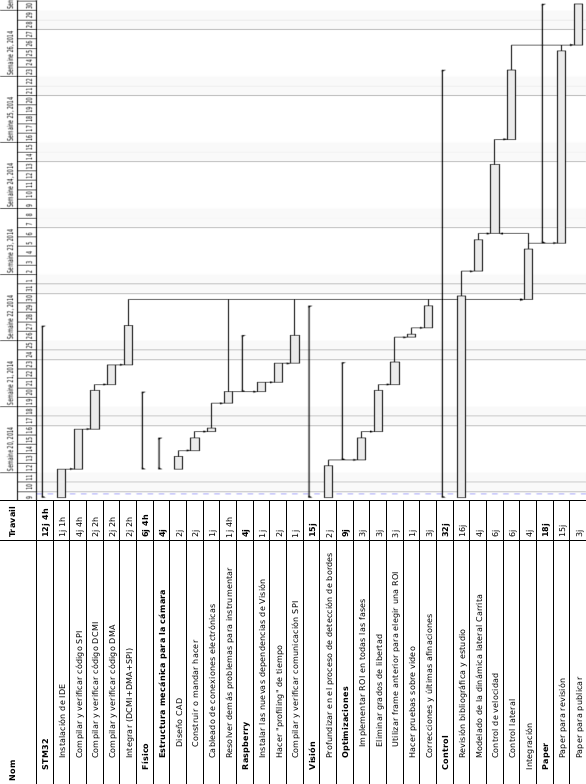
\includegraphics[height=1.3\textwidth]{fig/ganttscaled}\\
\caption{Gantt chart for the first two months.}
\label{fig_ganttA}
\end{center}
\end{figure}

\subsection{Camera mount mechanism drawings}
\begin{figure}[ht!]
\begin{center}
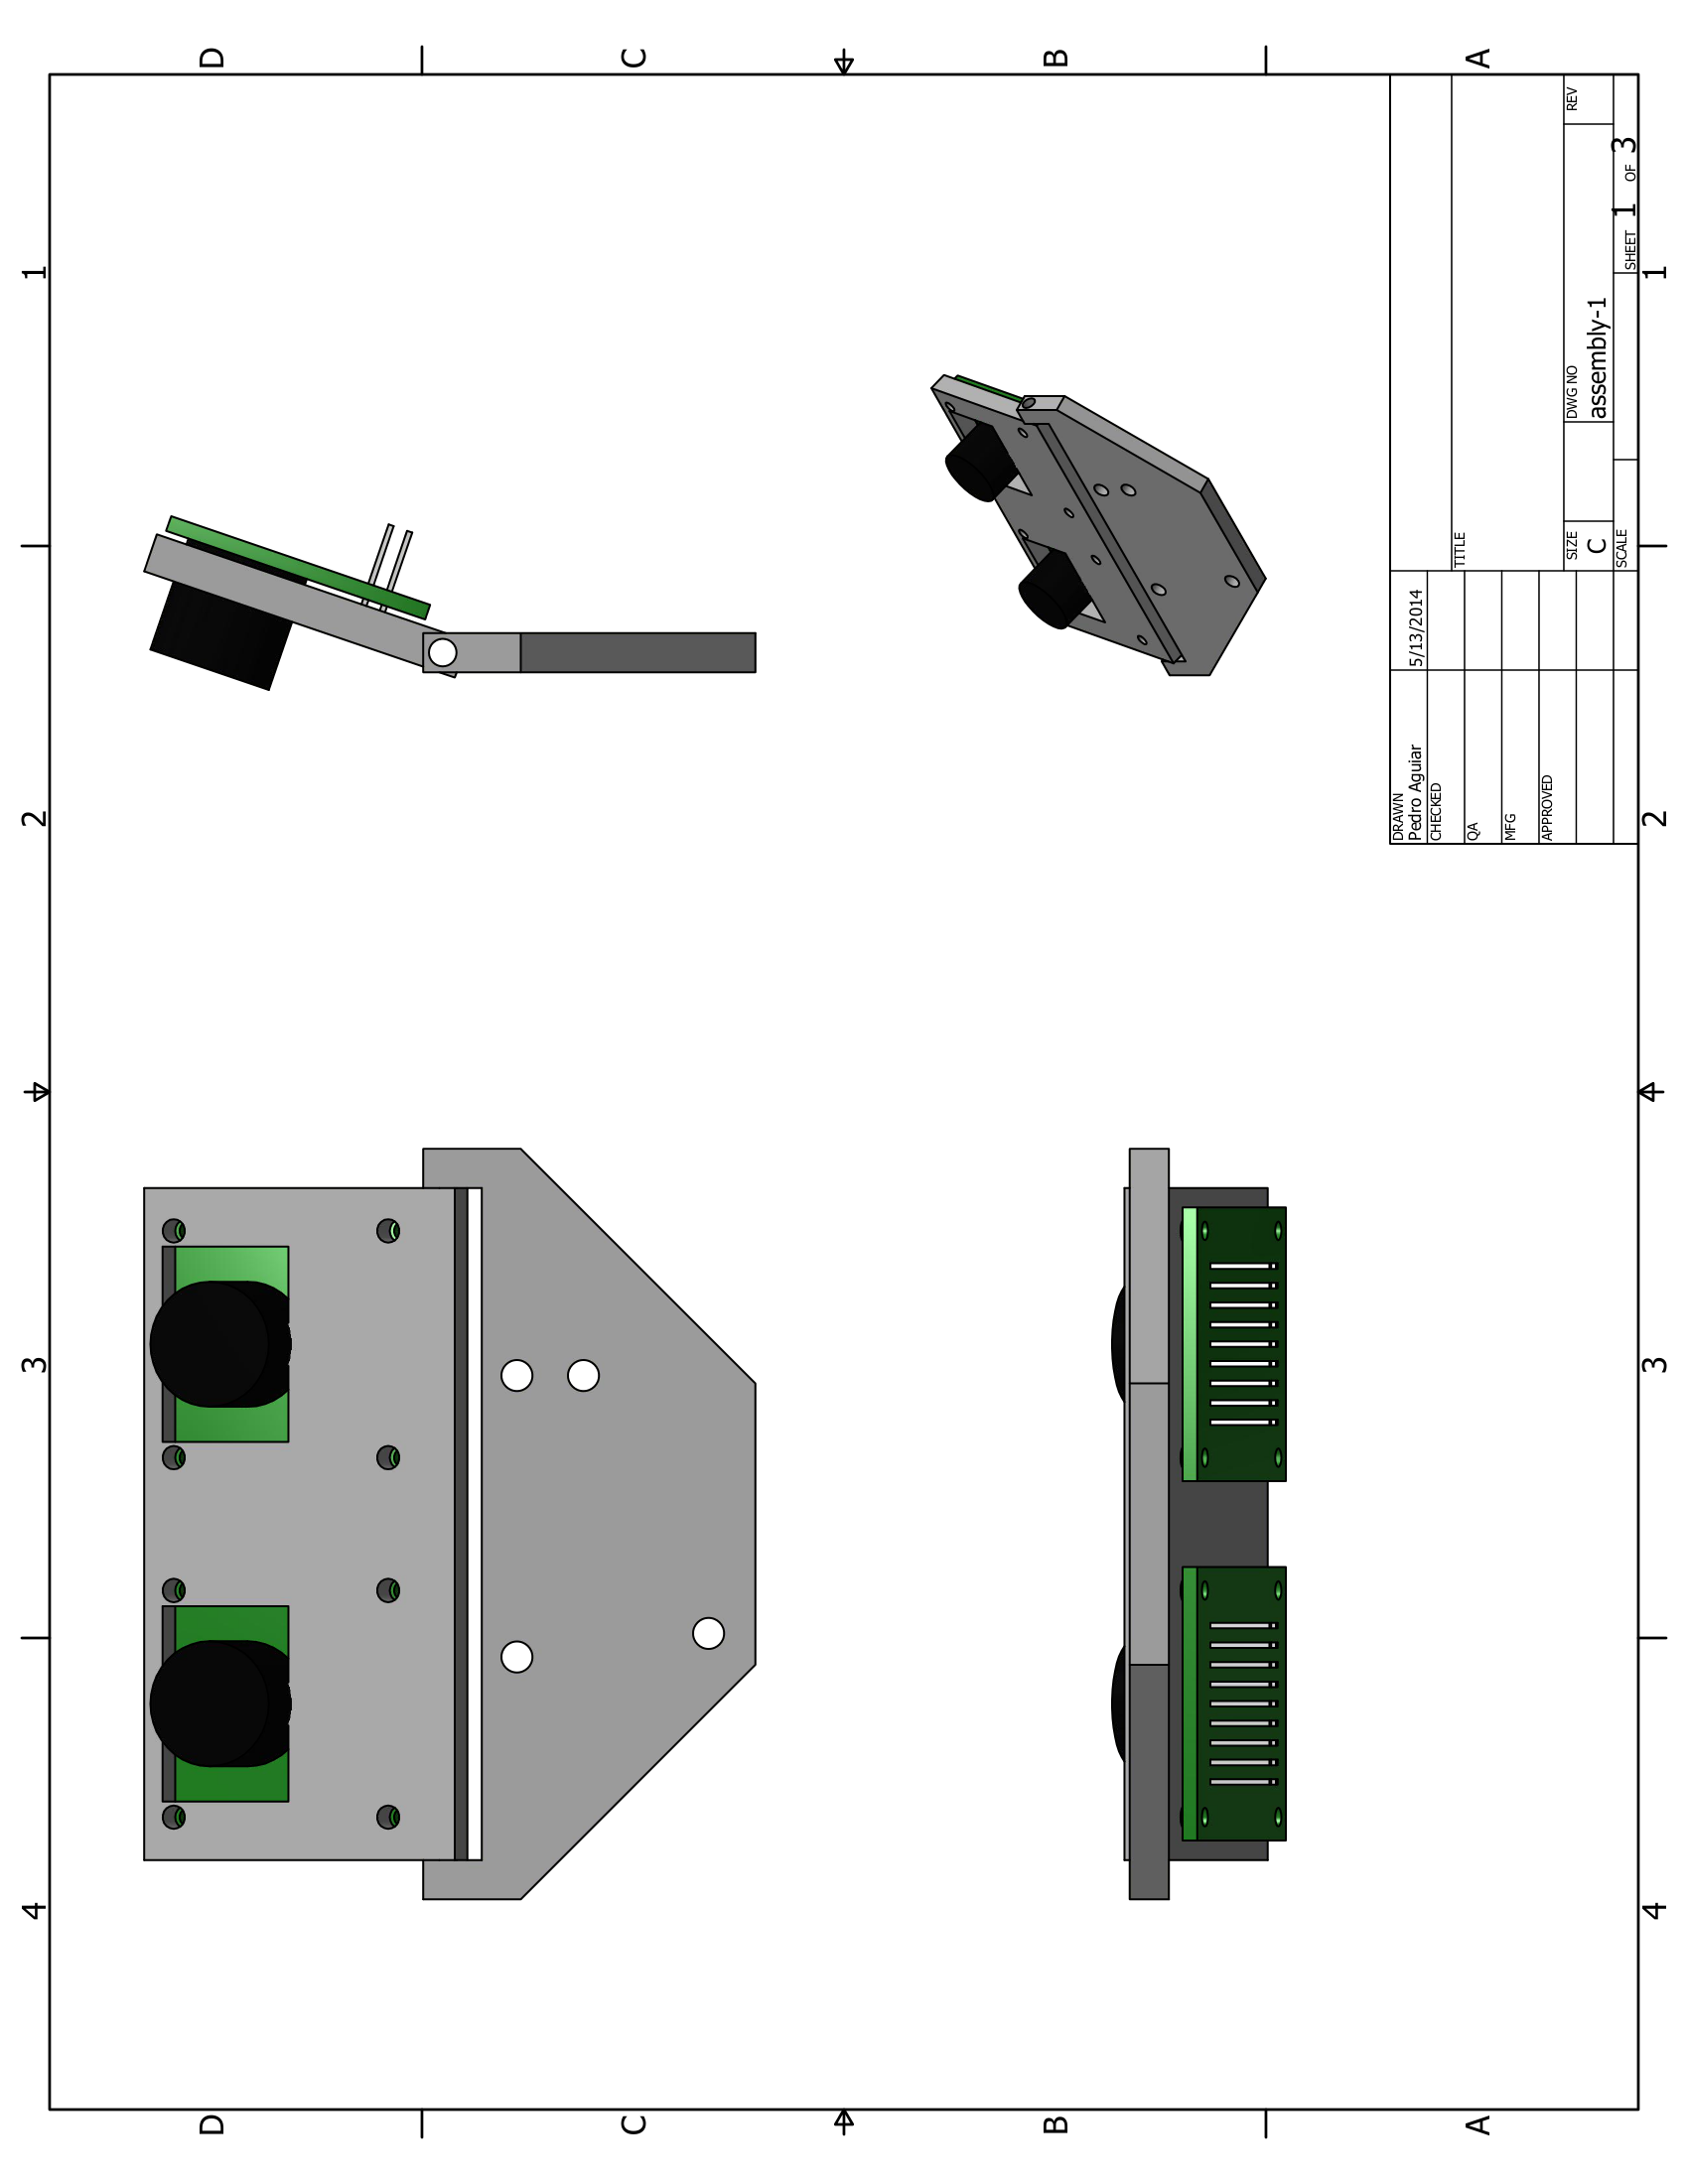
\includegraphics[height=1.2\textwidth]{fig/cammountp1}\\
\caption{Camera mount mechanism drawings: Assembled camera mount.}
\label{fig_cammountp1}
\end{center}
\end{figure}

\begin{figure}[ht!]
\begin{center}
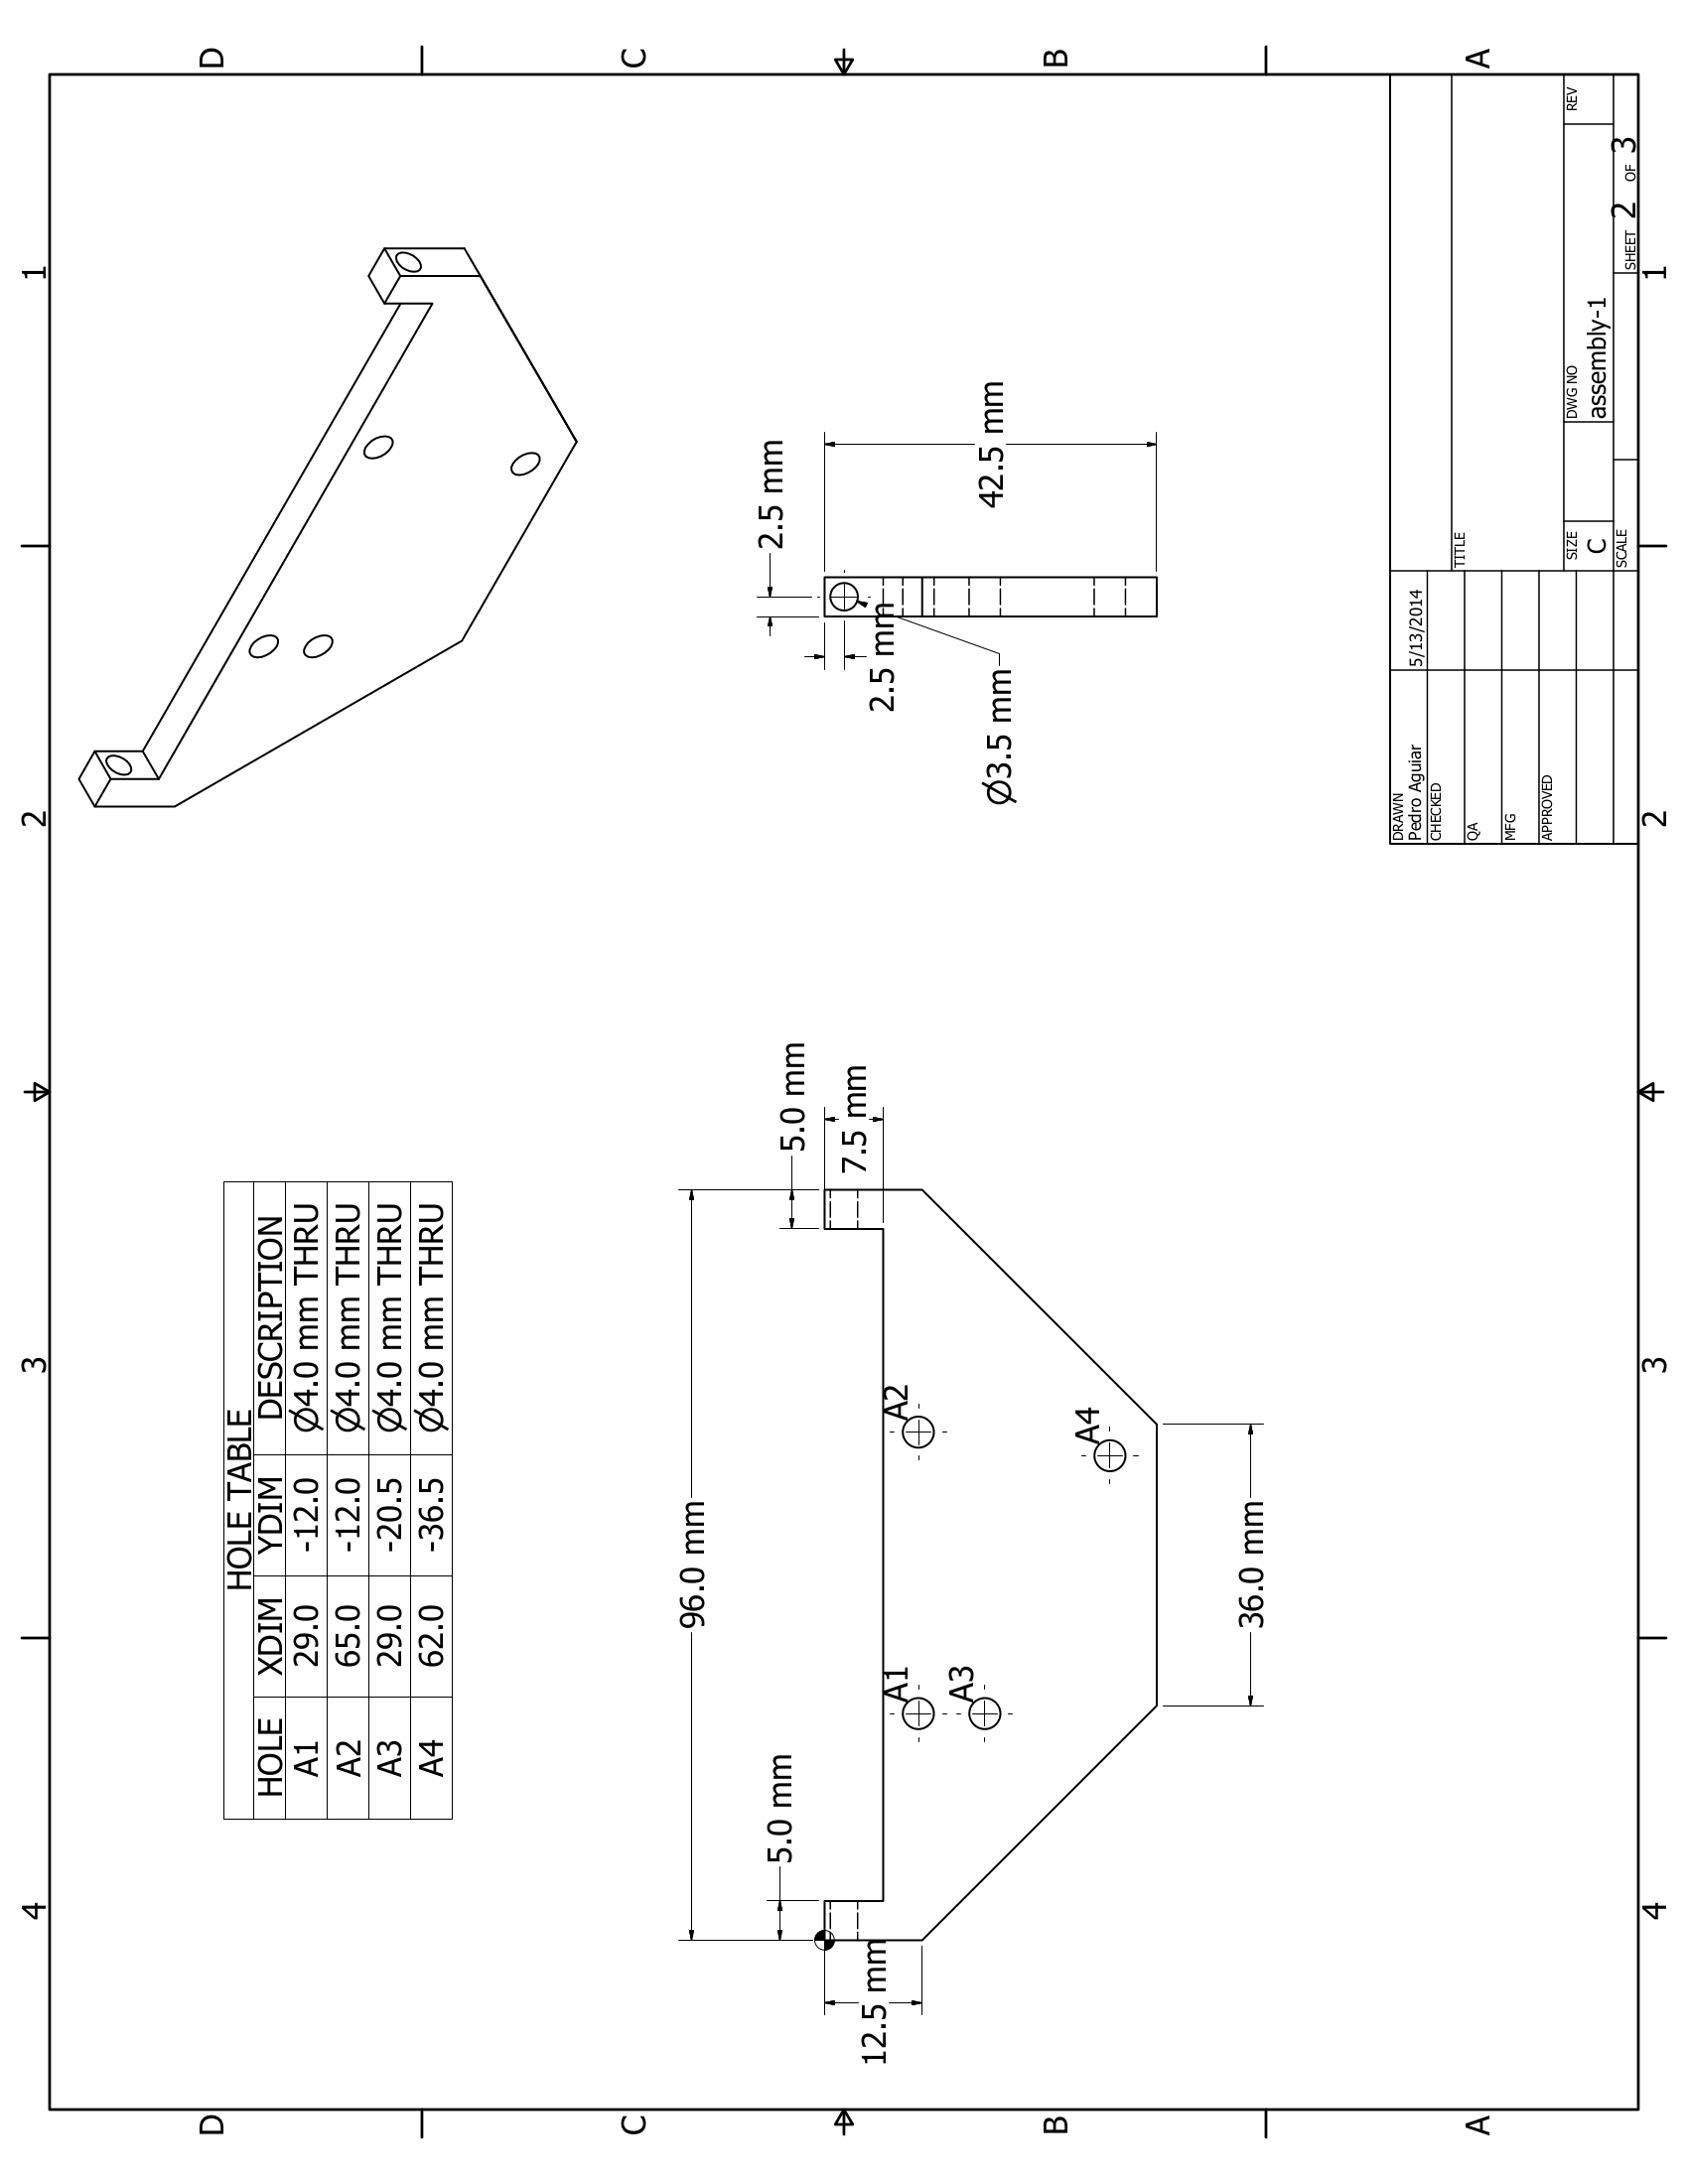
\includegraphics[height=1.2\textwidth]{fig/cammountp2}\\
\caption{Camera mount mechanism drawings: camera part.}
\label{fig_cammountp2}
\end{center}
\end{figure}

\begin{figure}[ht!]
\begin{center}
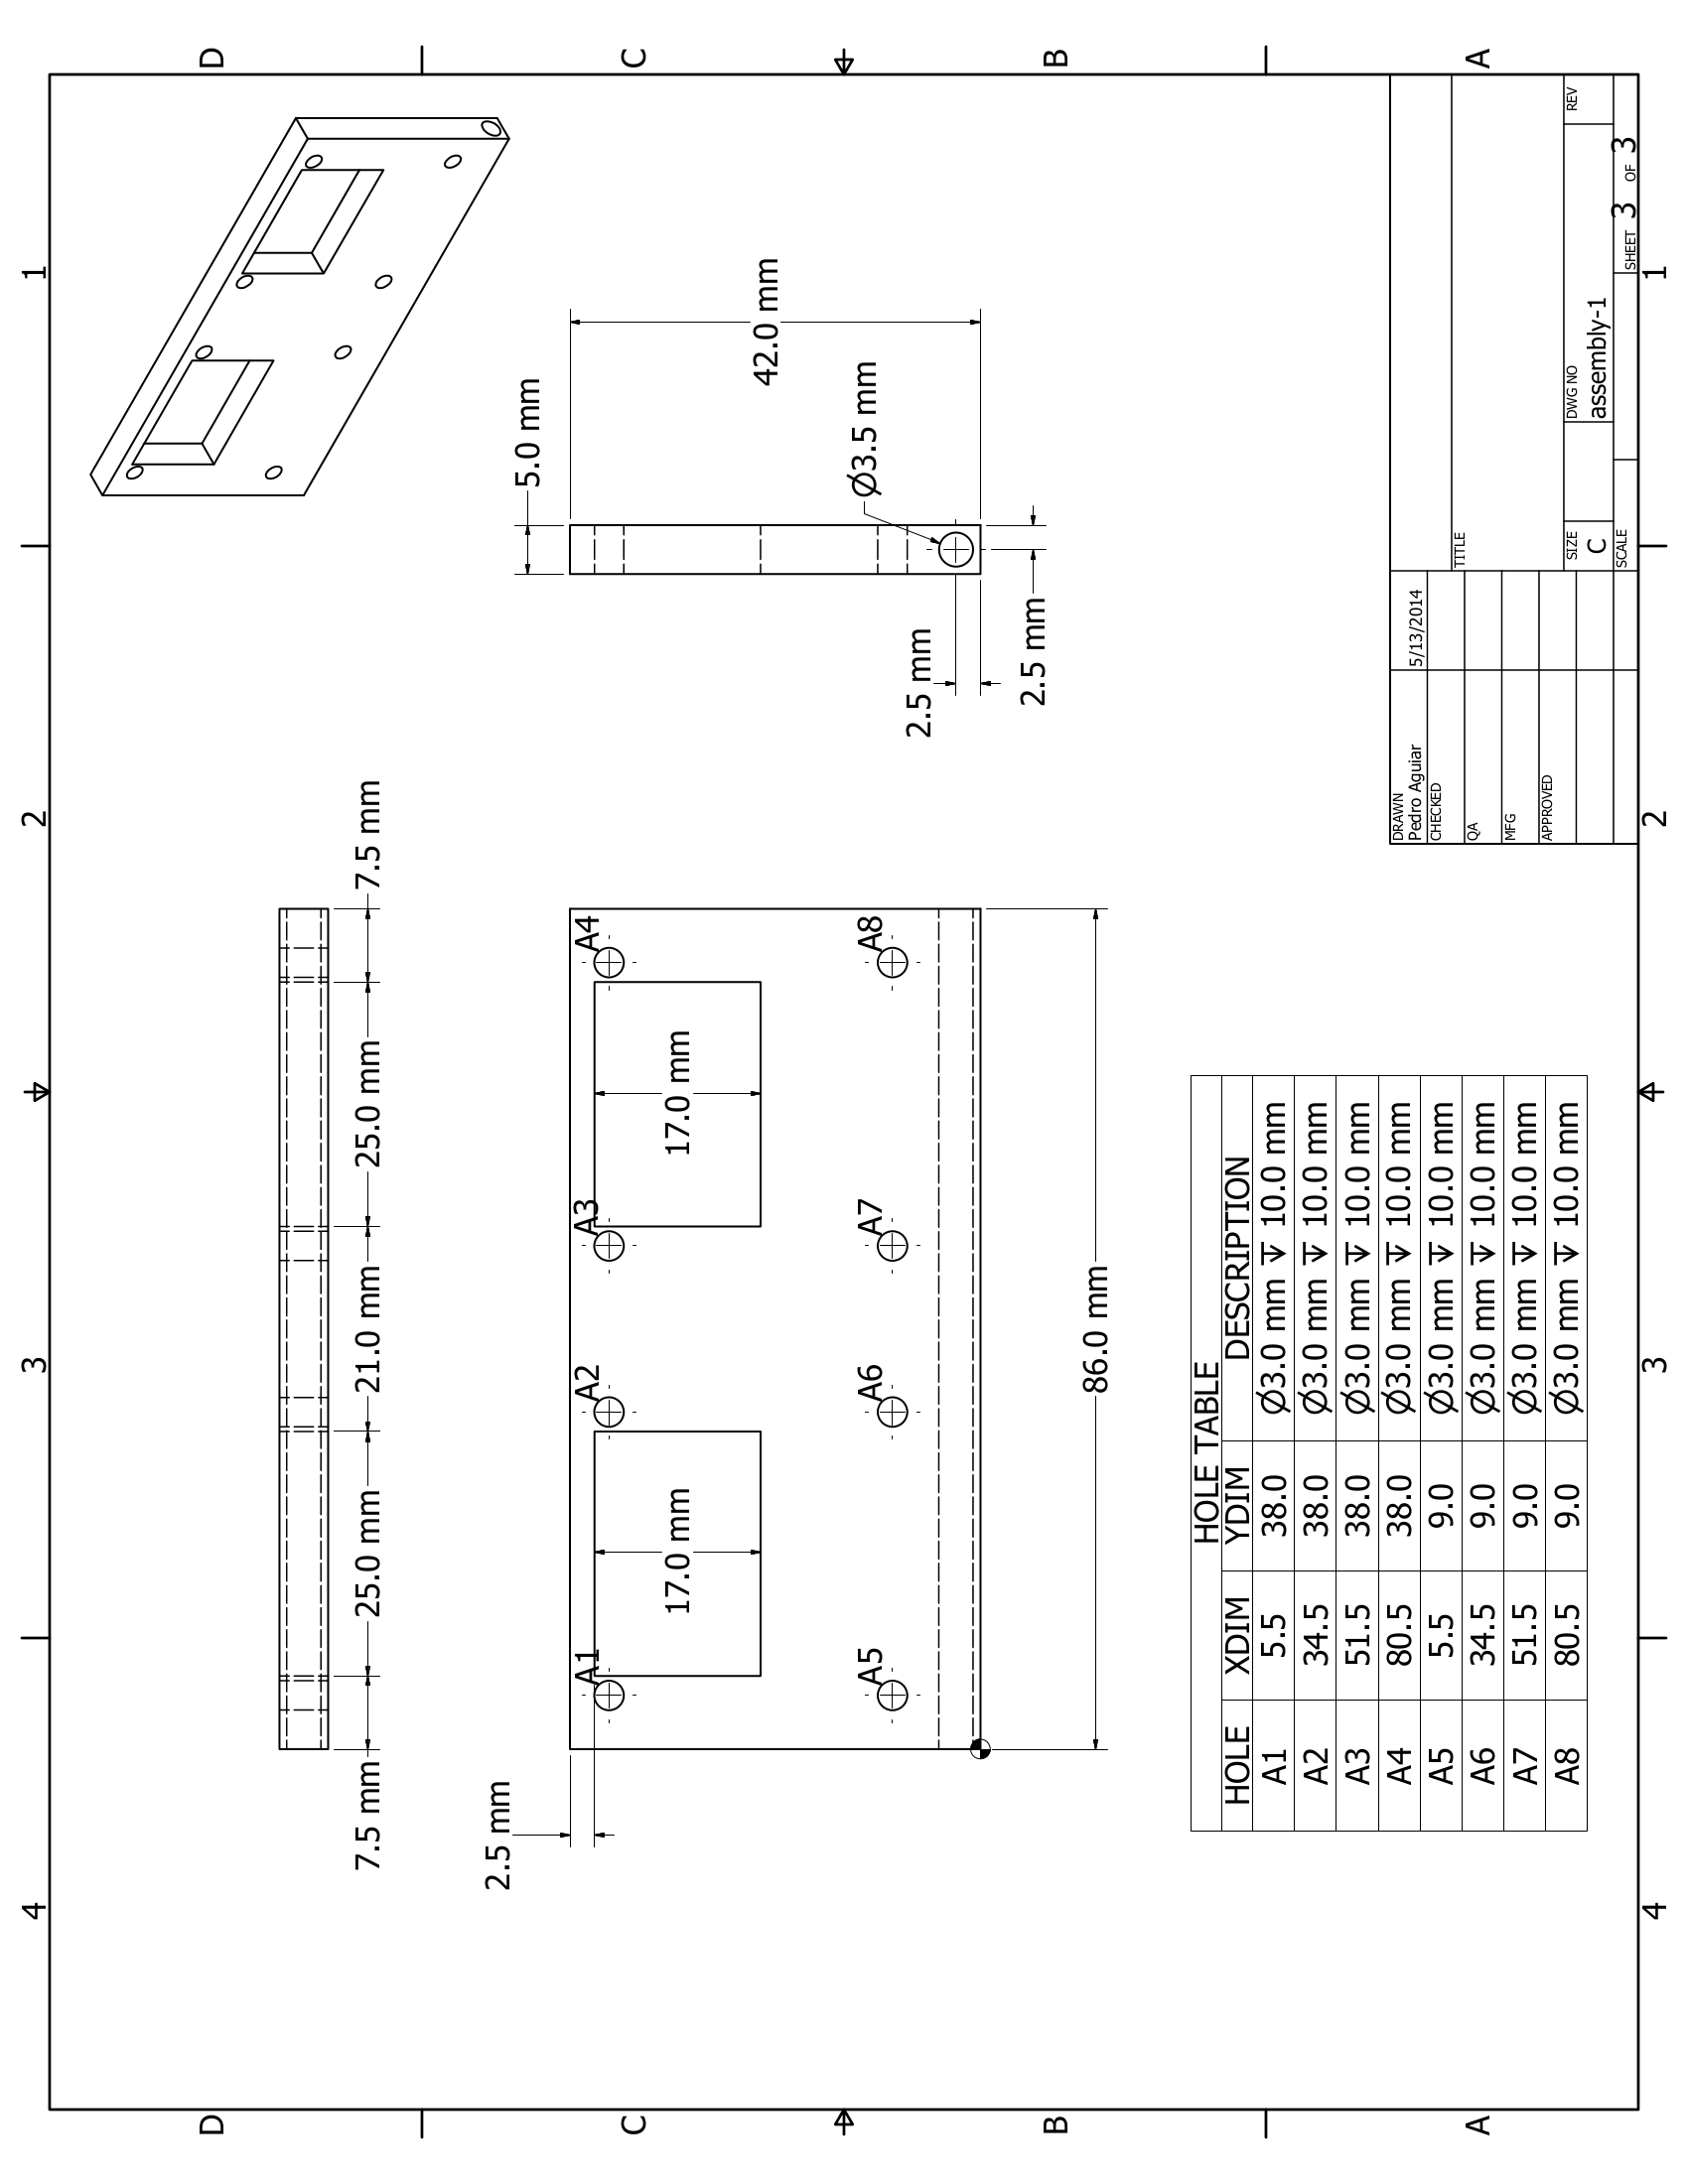
\includegraphics[height=1.2\textwidth]{fig/cammountp3}\\
\caption{Camera mount mechanism drawings: Carrita's part.}
\label{fig_cammountp3}
\end{center}
\end{figure}

\clearpage

\begin{thebibliography}{9}
 \bibitem{cummings}
	Chris Cummings,
	\emph{Gpu accelerated image processing on raspberry pi}. http://youtu.be/yQZISXIFjaQ

 \bibitem{dubska}
	Markéta Dubská, Adam Herout,
	\emph{Real-Time Detection of Lines using Parallel Coordinates and OpenGL}. 

\end{thebibliography}

\end{document}
